\documentclass[../../../main.tex]{subfiles}

\begin{document}
\subsection*{Lorentz Force Law}
\subsubsection*{Magnetic forces.} The magnetic force on a charge $Q$, moving with velocity $\mathbf{v}$ in a magnetic field \textbf{B}, is 
\begin{equation*}
    \mathbf{F}_{\text{mag}} = Q(\mathbf{v} \times \mathbf{B})
\end{equation*}
This is known as the Lorentz force law. In the presence of both electric and magnetic fields, the net force on $Q$ would be
\begin{equation*}
    \mathbf{F}= Q(\mathbf{E}+\mathbf{v} \times \mathbf{B})
\end{equation*}

One implication of the Lorentz force law deserves special attention
\begin{equation*}
\boxed{
    \textbf{Magnetic forces do no work.}
    }
\end{equation*}
For if $Q$ moves an amount $d\mathbf{l} = \mathbf{v} \;dt$, the work done is
\begin{equation*}
    dW_{\text{mag}} = \mathbf{F}_{\text{mag}} \cdot d\mathbf{l} = Q(\mathbf{v} \times \mathbf{B}) \cdot \mathbf{v} \;dt = 0
\end{equation*}
This follows because $\mathbf{v} \times \mathbf{B}$ is perpendicular to $\mathbf{v}$. Magnetic forces may alter the direction in which a particle moves, but they cannot speed it up or slow it down.

\subsubsection*{Current.} The current in a wire is the charge per unit time passing a given point. A line charge $\lambda$ traveling down a wire at speed \textbf{v} constitutes a current
\begin{equation*}
    \mathbf{I}=\lambda\mathbf{v}
\end{equation*}

The magnetic force on a segment of current-carrying wire is
\begin{equation*}
    \mathbf{F}_{\text{mag}}=\int (\mathbf{v} \times \mathbf{B}) dq=\int (\mathbf{v} \times \mathbf{B}) \lambda\; dl
\end{equation*}
thus
\begin{equation*}
    \mathbf{F}_{\text{mag}}=\int (\mathbf{I}\times \mathbf{B})\;dl
\end{equation*}
Inasmuch as $\mathbf{I}$ and $d\mathbf{l}$ both point in the same direction, we can just as well write 
this as
\begin{equation*}
    \mathbf{F}_{\text{mag}}=I\int (d\mathbf{l}\times \mathbf{B})
\end{equation*}
where the current is constant (in magnitude) along the wire.

\subsubsection*{Surface current density.} Consider a “ribbon” of infinitesimal width $dl\bot$, running parallel to the flow. If the current in this ribbon is $d\mathbf{I}$, the surface current density is
\begin{equation*}
    \mathbf{K}\equiv\frac{d\mathbf{I}}{dl\bot}
\end{equation*}
In words, $\mathbf{K}$ is the current per unit width. In particular, if the (mobile) surface charge density is $\sigma$ and its velocity is $\mathbf{v}$, then
\begin{equation*}
    \mathbf{K}\equiv\sigma\mathbf{v}
\end{equation*}
The magnetic force on the surface current is
\begin{equation*}
    \mathbf{F}_{\text{mag}}=\int (\mathbf{v}\times\mathbf{B})\sigma\;da= \int (\mathbf{K}\times\mathbf{B})\;da
\end{equation*}

\subsubsection*{Volume current density.} Consider a tube of infinitesimal cross-section $da\bot$, running parallel to the flow. If the current in this tube is $d\mathbf{I}$, the volume current density is
\begin{equation*}
    \mathbf{J}\equiv\frac{d\mathbf{I}}{da\bot}
\end{equation*}
In words, $\mathbf{J}$ is the current per unit area. If the (mobile) volume charge density is $\rho$ and the velocity is $\mathbf{v}$, then
\begin{equation*}
    \mathbf{J}\equiv\rho\mathbf{v}
\end{equation*}
The magnetic force on a volume current is therefore
\begin{equation*}
    \mathbf{F}_{\text{mag}}=\int (\mathbf{v}\times\mathbf{B})\rho\;d\tau= \int (\mathbf{J}\times\mathbf{B})\;d\tau
\end{equation*}

\begin{figure*}
    \centering
    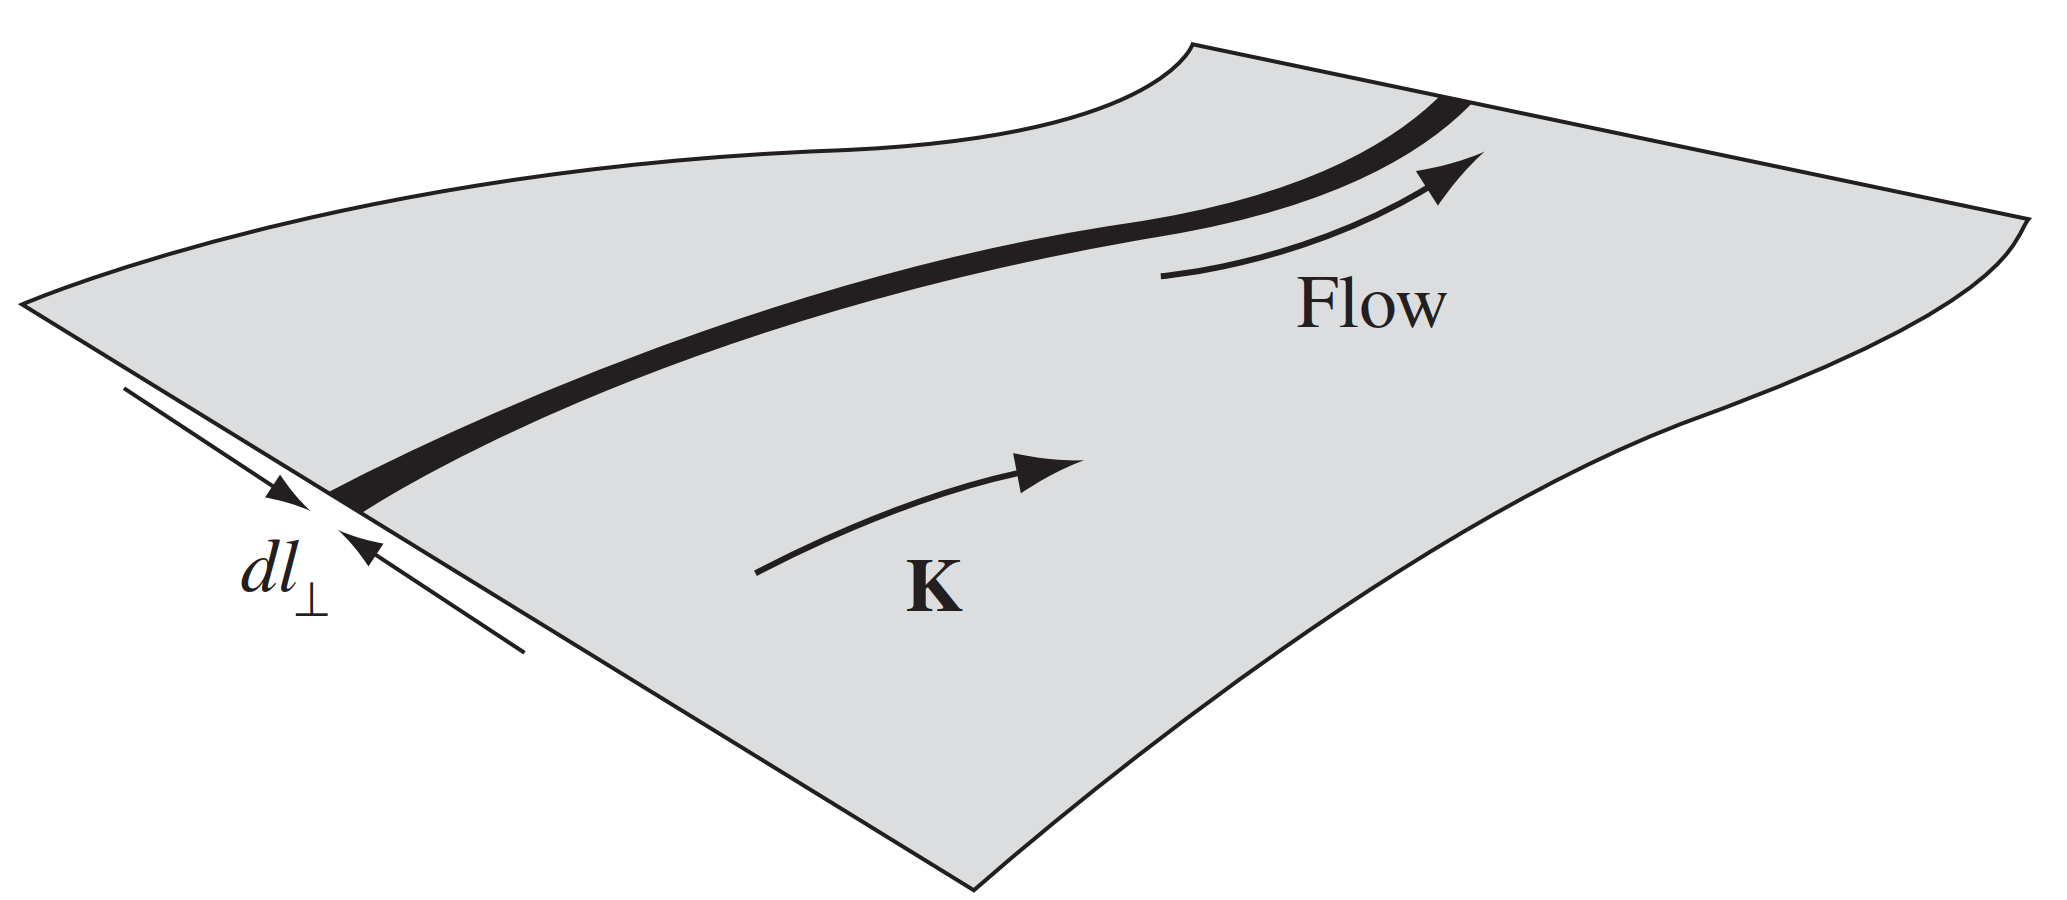
\includegraphics[width=0.4\textwidth]{../Rss/Electromagnetism/Magnetostatics/SurfCurrent}
    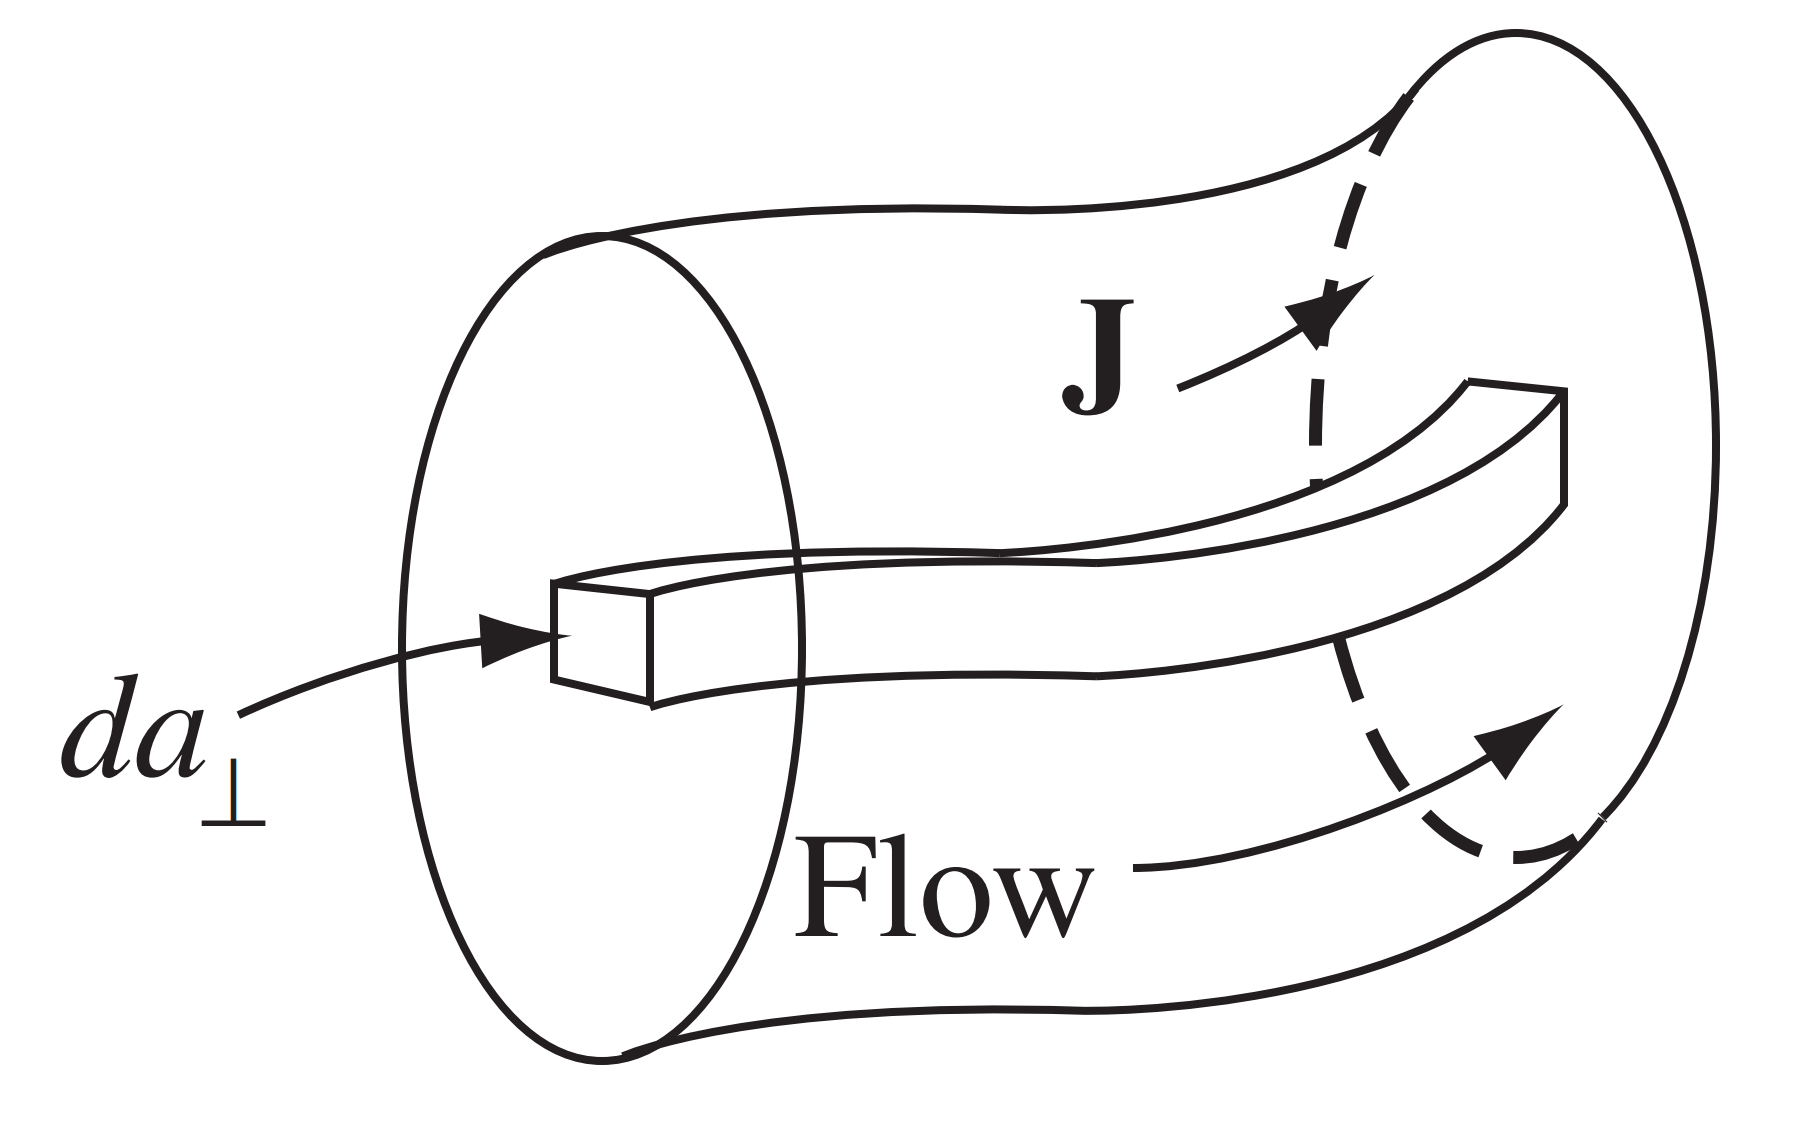
\includegraphics[width=0.4\textwidth]{../Rss/Electromagnetism/Magnetostatics/VolCurrent}
    \caption*{Figure: surface and volume current.}
\end{figure*}


\subsubsection*{Continuity equation.} From the definition of volume current, the total current crossing a surface $\mathcal{S}$ can be written as
\begin{equation*}
    I=\int_{\mathcal{S}}\mathbf{J}\cdot d\mathbf{a}
\end{equation*}
In particular, the charge per unit time leaving a volume $\mathcal{V}$ is
\begin{equation*}
    \oint_{\mathcal{S}} \mathbf{J}\cdot d\mathbf{a}=\int_{\mathcal{V}}(\nabla\cdot\mathbf{J}) \;d\tau
\end{equation*}
Because charge is conserved, whatever flows out through the surface must come at the expense of what remains inside:
\begin{equation*}
    \int_{\mathcal{V}}(\nabla\cdot\mathbf{J}) \;d\tau=-\frac{d}{dt}\int_\mathcal{V}\rho\;d\tau= -\int_\mathcal{V}\frac{d\rho}{dt}\;d\tau
\end{equation*}
where minus sign reflects the fact that an outward flow decreases the charge left in $\mathcal{V}$. Since this applies to any volume, we conclude that
\begin{equation*}
    \nabla\cdot\mathbf{J}=-\frac{d\rho}{dt}
\end{equation*}
This is the precise mathematical statement of local charge conservation; it is called the continuity equation.

\subsubsection*{Dictionary.} For future reference, let me summarize the “dictionary” we have implicitly developed for translating equations into the forms appropriate to point, line, surface, and volume currents:
\begin{equation*}
    \sum_{n=1}^{n}q_i\mathbf{v}_i\sim\int_\mathcal{L}\mathbf{I}\;dl \sim \int_\mathcal{S}\mathbf{K}\;da \sim \int_\mathcal{V}\mathbf{J}\;d\tau
\end{equation*}

\subsection*{Biot-Savart Law}
Steady currents produce magnetic fields that are constant in time; the theory of steady currents is called magnetostatics. By steady current I mean a continuous flow that has been going on forever, without change and without charge piling up anywhere. Formally, electro/magnetostatics is the régime
\begin{equation*}
    \frac{\partial\rho}{\partial t}=0 \quad\frac{\partial \mathbf{J}}{\partial t}=0
\end{equation*}

At all places and all times. Notice that a moving point charge cannot possibly constitute a steady current. 

When a steady current flows in a wire, its magnitude I must be the same all along the line. More generally, since $\partial\rho/\partial t=0$ in magnetostatics, the continuity equation becomes
\begin{equation*}
    \nabla\cdot \mathbf{J}=0
\end{equation*}

\subsubsection*{Biot-Savart law.} The magnetic field of a steady line current is given by the Biot-Savart law 
\begin{equation*}
    \mathbf{B}(\mathbf{r})=\frac{\mu_0}{4\pi}\int \frac{\mathbf{I} \times\hrcurs}{\rcurs^2}dl'=\frac{\mu_0I}{4\pi}\int \frac{d \mathbf{l} \times\hrcurs}{\rcurs^2}
\end{equation*}
The integration is along the current path, in the direction of the flow; $d\mathbf{l}'$ is an element of length along the wire, and $\brcurs$, as always, is the vector from the source to the point $\mathbf{r}$.
The constant $\mu_0$ is called the permeability of free space:
\begin{equation*}
    \mu_0=4\pi \times 10^{-7} \quad \text{N/A}^2
\end{equation*}
\begin{figure*}[ht]
    \centering
    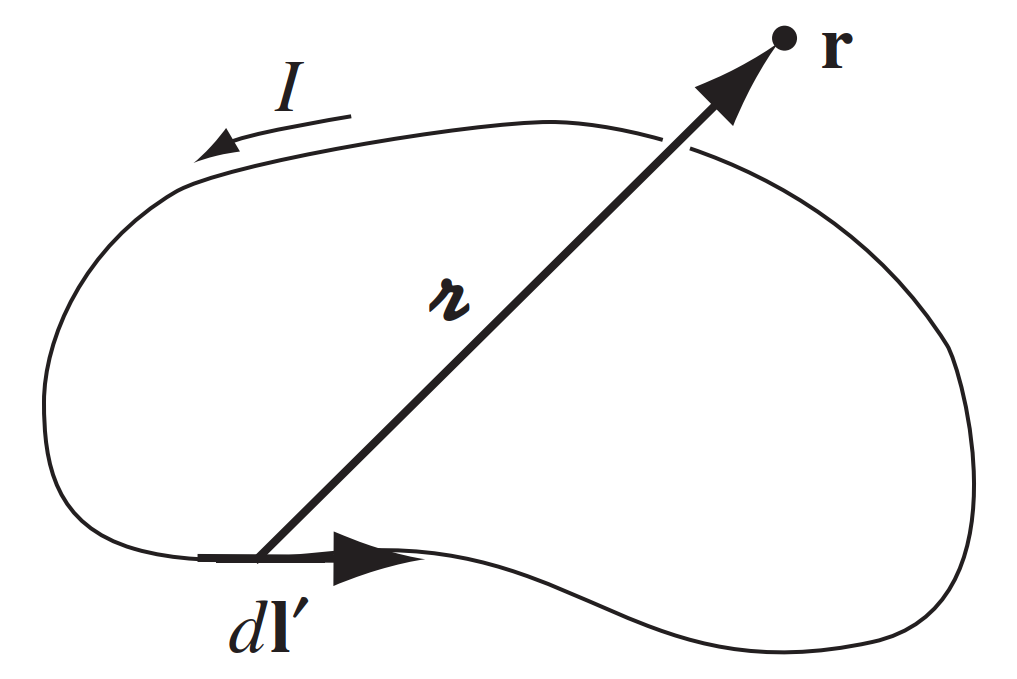
\includegraphics[width=0.3\textwidth]{../Rss/Electromagnetism/Magnetostatics/BiotSavart}
\end{figure*}

\subsection*{The Hall Effect} 
\begin{figure*}[t]
    \centering
    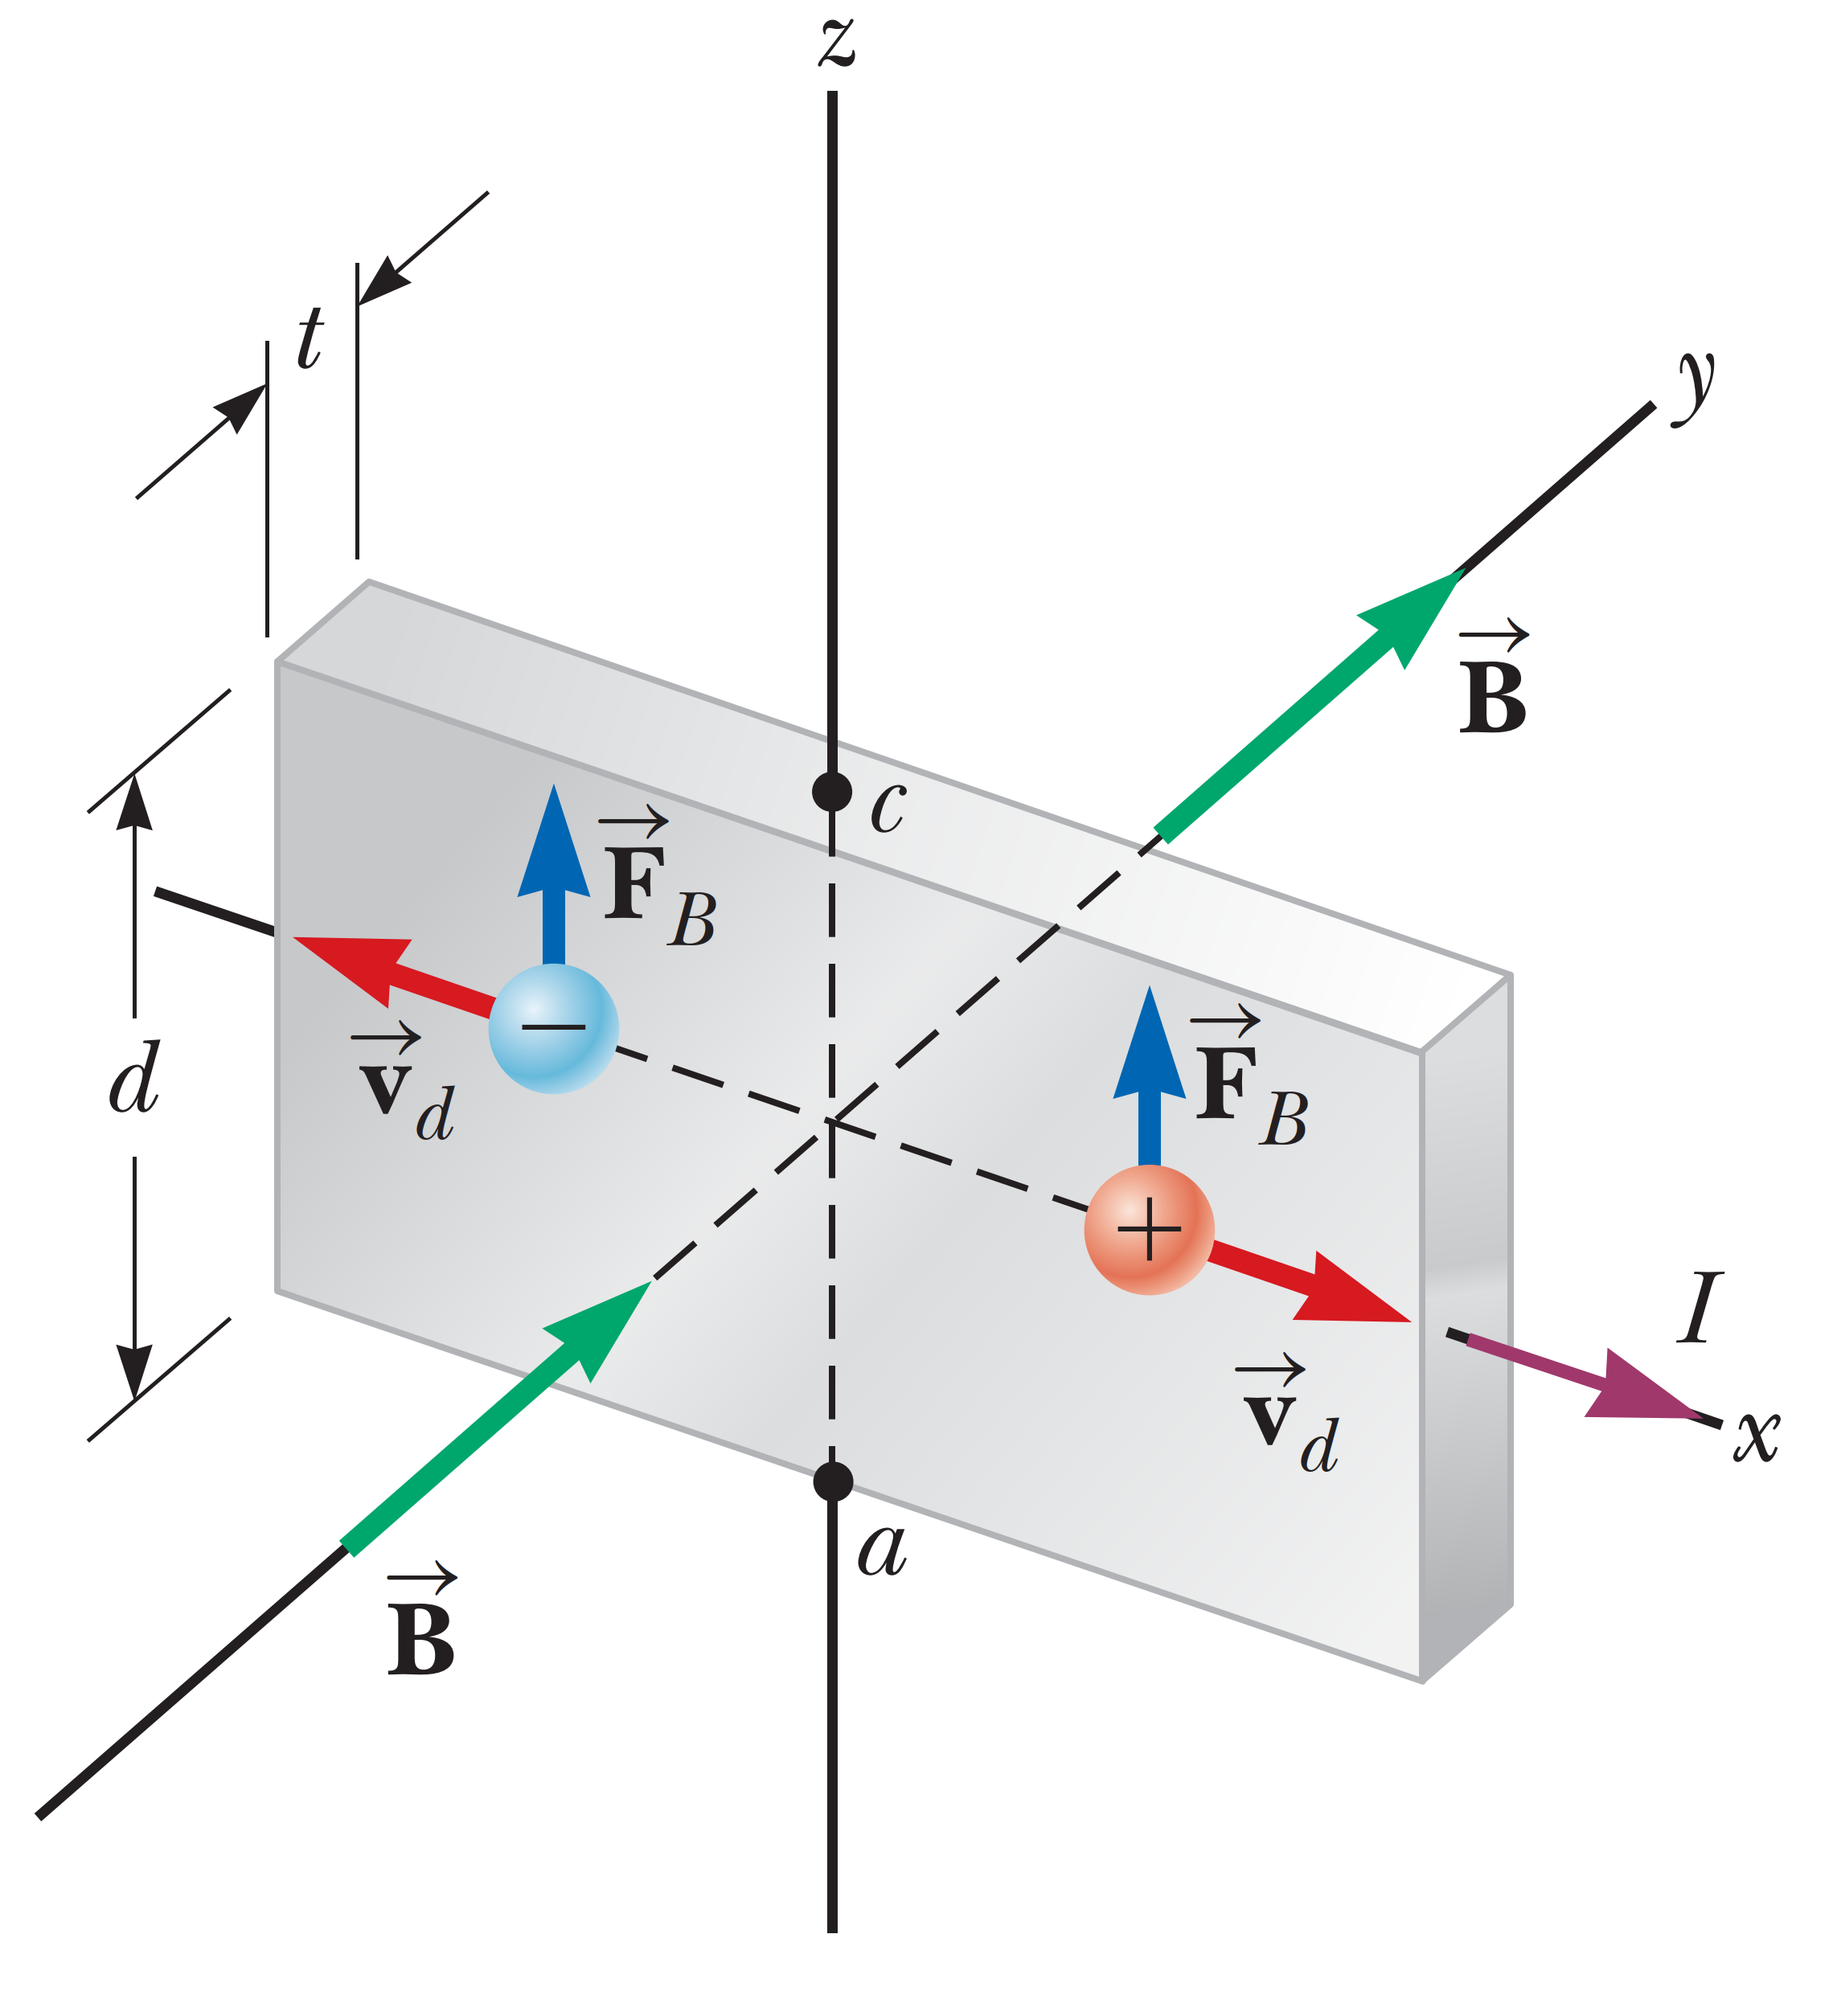
\includegraphics[width=0.5\textwidth]{../Rss/Electromagnetism/Magnetostatics/HallEffect}
    \caption*{Figure: arrangement of the Hall effect}
\end{figure*}
The phenomenon known as the Hall effect occur when a current-carrying conductor is placed in a magnetic field, a potential difference is generated in a direction perpendicular to both the current and the magnetic field. The arrangement itself consists of a flat conductor carrying a current $I$ in the $x$ direction, with a uniform magnetic field \textbf{B} is applied in the $y$ direction. If the charge carriers are electrons moving in the negative $x$ direction with a drift velocity $\mathbf{v}_d$, they experience an upward magnetic force $\mathbf{F}=-q\mathbf{v}_d\times\mathbf{B}$, and are deflected upward. This accumulation of charge at the edges establishes an electric field in the conductor and increases until the electric force on carriers remaining in the bulk of the conductor balances the magnetic force acting on the carriers. In equilibrium, the magnetic is balanced by the electric force, therefore
\begin{align*}
    -qv_dB&=-qE_H\\
    E_H=v_dB
\end{align*}
If $d$ is the width of the conductor, the Hall voltage is
\begin{equation*}
    V_H=E_Hd=v_dBd
\end{equation*}
Since infinitesimal charge $dq$ inside infinitesimal length $dx$ inside conductors can be expressed as $dq=qnAdx=qnAv_ddt$
\begin{equation*}
    V_H=\frac{IBd}{nqA}=\frac{IB}{nqt}=\frac{IB}{t}R_H
\end{equation*}
where $R_H=1/nq$ is called the Hall coefficient. This relationship shows that a properly calibrated conductor can be used to measure the magnitude of an unknown magnetic field. 

\subsection*{Divergence and Curl of Magnetic Field}
\subsubsection*{Curl.} Magnetic field of an infinite straight wire is
\begin{equation*}
    \mathbf{B}=\frac{\mu_0I}{2\pi s}\boldsymbol{\hat{\phi}}
\end{equation*}
The integral of \textbf{B} around a circular path of radius $s$, centered at the wire, is
\begin{equation*}
    \oint \mathbf{B}\cdot d\mathbf{l}=\oint\frac{\mu_0I}{2\pi s}dl=\mu_0I
\end{equation*}
Notice that the answer is independent of $s$; that's because \textbf{B} decreases at the same rate as the circumference increases. With more work, you can generalize for any arbitrary wire and get the same result. 

Now suppose we have a bundle of straight wires. Each wire that passes through our loop contributes $\mu_0 I$, and those outside contribute nothing. The line integral will then be
\begin{equation*}
    \oint \mathbf{B}\cdot d\mathbf{l}=\mu_0I_{\text{enc}}
\end{equation*}
where $I_{\text{enc}}$ stands for the total current enclosed by the integration path. If the flow 
of charge is represented by a volume current density, the enclosed current is
\begin{equation*}
    I_{\text{enc}}=\int \mathbf{J}\cdot d\mathbf{a}
\end{equation*}
Using Stokes' theorem, we can write 
\begin{align*}
    \oint \mathbf{B}\cdot d\mathbf{l}&=\mu_0I_{\text{enc}}\\
    \int(\nabla \times \mathbf{B})\cdot d\mathbf{a}&=\mu_0\int \mathbf{J}\cdot d\mathbf{a}
\end{align*}
and hence
\begin{equation*}
    \nabla \times \mathbf{B}=\mu_0\mathbf{J} 
\end{equation*}

Most current configurations cannot be constructed out of infinite straight wires, so the next section is devoted to the formal derivation of the divergence and curl of B, starting from the Biot-Savart law itself.

\subsubsection*{Divergence.} Evidently the divergence of the magnetic field is
\begin{equation*}
    \nabla \cdot \mathbf{B}=0
\end{equation*}

\subsection*{Ampere's Law}
The equation for the curl of \textbf{B}
\begin{equation*}
    \nabla\times \mathbf{B}=\mu_0 \mathbf{J}
\end{equation*}
is called Ampère’s law (in differential form). It can be converted to integral form by the usual device of applying one of the fundamental theorems—in this case Stokes’ theorem
\begin{equation*}
    \int(\nabla\times \mathbf{B})\cdot d\mathbf{a}=\oint \mathbf{B}\cdot d\mathbf{l}
\end{equation*}
Thus
\begin{equation*}
    \oint \mathbf{B}\cdot d\mathbf{l}=\mu_0\int\mathbf{J} \cdot d\mathbf{a}
\end{equation*}
Since $\int\mathbf{J} \cdot d\mathbf{a}$ is the total current passing through the surface which we call $I_{\text{enc}}$ 
\begin{equation*}
    \oint \mathbf{B}\cdot d\mathbf{l}=\mu_0I_{\text{enc}}
\end{equation*}
Like Gauss’s law, Ampère’s law is always true (for steady currents), but it is not always useful. The current configurations that can be handled by Ampère’s law are Infinite straight lines, Infinite planes, Infinite solenoids, Toroids. 

\subsection*{Magnetic Vector Potential}
Just as $\nabla \times \mathbf{E}=0$ permitted us to introduce a scalar potential ($V $) in electrostatics $\mathbf{E}=-\nabla V $, so $\nabla \cdot \mathbf{B}=0 $ invites the introduction of a vector potential \textbf{A} in magnetostatics
\begin{equation*}
    B=\nabla\times \mathbf{ A}
\end{equation*}
The potential formulation automatically takes care of $\nabla \cdot\mathbf{B} = 0$ (since the divergence of a curl is always zero); there remains Ampère’s law:
\begin{align*}
    \nabla\times\mathbf{B}&=\mu_0\mathbf{J}\\
    \nabla\times\nabla\times \mathbf{ A}&=\mu_0\mathbf{J}\\
    \nabla(\nabla\cdot\mathbf{B}) - \nabla^2 \mathbf{A}&=\mu_0\mathbf{J}\\
\end{align*}
With $\mathbf{A}$, Ampère’s law becomes
\begin{equation*}
    \nabla^2 \mathbf{A}=-\mu_0\mathbf{J}
\end{equation*}
This again is nothing but Poisson’s equation—or rather, it is three Poisson’s equations, one for each Cartesian component. Assuming \textbf{J} goes to zero at infinity, we can read off the solution
\begin{equation*}
    \mathbf{A}(\mathbf{r})=\frac{\mu_0}{4\pi}\int\frac{\mathbf{J}(\mathbf{r'})}{\rcurs}d\tau'
\end{equation*}
For line current
\begin{equation*}
    \mathbf{A}(\mathbf{r})=\frac{\mu_0}{4\pi}\int\frac{\mathbf{I}}{\rcurs}dl'=\frac{\mu_0I}{4\pi}\int\frac{1}{\rcurs}d\mathbf{l'}
\end{equation*}
and surface currents
\begin{equation*}
    \mathbf{A}(\mathbf{r})=\frac{\mu_0}{4\pi}\int\frac{\mathbf{K}(\mathbf{r'})}{\rcurs}da'
\end{equation*}

\subsection*{Multipole Expansion}
If you want an approximate formula for the vector potential of a localized current distribution, valid at distant points, a multipole expansion is in order. As we found
\begin{equation*}
    \frac{1}{\rcurs}=\frac{1}{r}\sum_{n=0}^{\infty} \biggl(\frac{r'}{r}\biggr)^nP_n(\cos\alpha)
\end{equation*}
where $\alpha$ is the angle between \textbf{r} and \textbf{r'}. Accordingly, the vector potential of a current loop can be written
\begin{equation*}
    \mathbf{A}(\mathbf{r})=\frac{\mu_0I}{4\pi}\sum_{n=0}^{\infty} \frac{1}{r^{n+1}}\oint r'^n P_n(\cos\alpha) \;d\mathbf{l}'
\end{equation*}
more explicitly
\begin{multline*}
    \mathbf{A}(\mathbf{r})=\frac{\mu_0I}{4\pi}\bigg[\frac{1}{r}\oint\;d\mathbf{l}'+\frac{1}{r^2}\oint r' \cos \alpha\;d\mathbf{l}' +\\ \frac{1}{r^3}\oint r'^2 \biggl(\frac{3}{2}\cos\alpha -\frac{1}{2}\biggr) \alpha\;d\mathbf{l}'+\dots \bigg]
\end{multline*}
As in the multipole expansion of $V$, we call the first term (which goes like $1/r$) the 
monopole term, the second dipole, the third quadrupole, and so on. Now, the magnetic monopole term is always zero, for the integral is just the total vector displacement around a closed loop. This reflects the fact that there are no magnetic monopoles in nature. 

\begin{figure*}
    \centering
    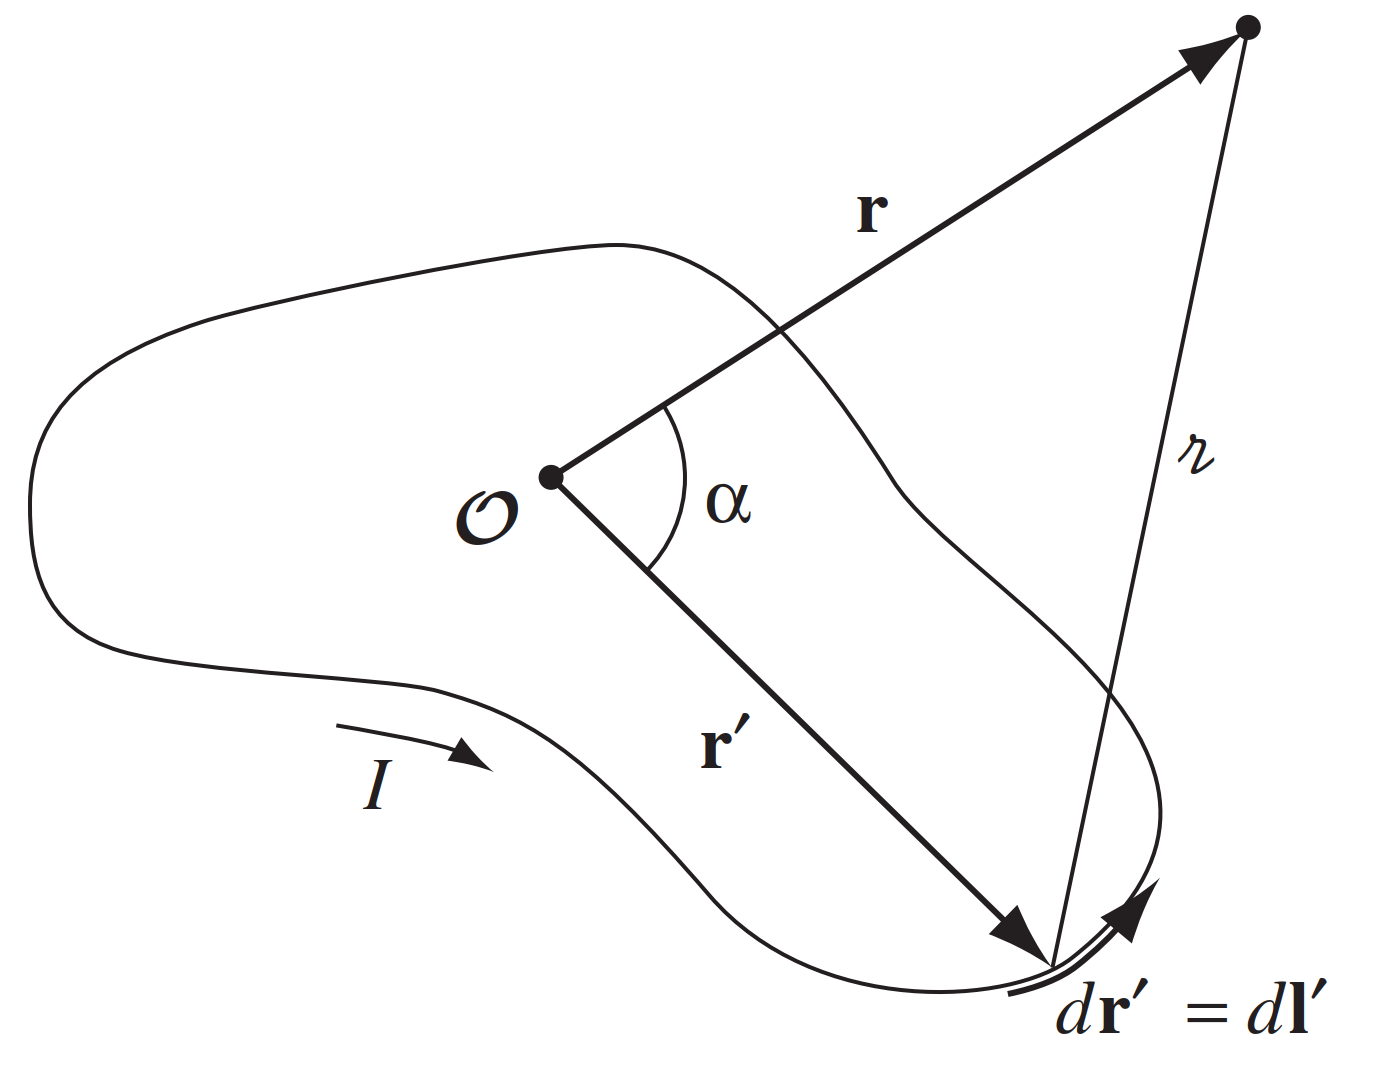
\includegraphics[width=0.5\textwidth]{../Rss/Electromagnetism/Magnetostatics/PolesExpansion}
\end{figure*}

In the absence of any monopole contribution, the dominant term is the dipole
\begin{equation*}
    \mathbf{A}_\text{dip}(\mathbf{r})=\frac{\mu_0I}{4\pi r^2}\oint r' \cos \alpha\;d\mathbf{l}'= \frac{\mu_0I}{4\pi r^2} \oint \mathbf{\hat{r}}\cdot\mathbf{r'}\;d\mathbf{l}'
\end{equation*}
This integral can be rewritten in a more illuminating way if we invoke
\begin{equation*}
    \oint  (\mathbf{c} \cdot \mathbf{r}) \;d\mathbf{l} =\biggl(\oint  \mathbf{r}\times d\mathbf{l }\biggr) \times \mathbf{c}
\end{equation*}
for any constant vector \textbf{c}. Then
\begin{equation*}
    \oint  (\mathbf{\hat{r}} \cdot \mathbf{r}) \;d\mathbf{l} = \int d\mathbf{a}'\times\mathbf{\hat{r}}
\end{equation*}
and 
\begin{equation*}
    \mathbf{A}_\text{dip}(\mathbf{r})=\frac{\mu_0 }{4\pi  }\frac{\mathbf{m}\times \mathbf{\hat{r}}}{r^2}
\end{equation*}
where \textbf{m} is the magnetic dipole moment
\begin{equation*}
    \mathbf{m}\equiv I\int d\mathbf{a}=I\mathbf{a}
\end{equation*}

\subsubsection*{Field of Dipole.} In practice, the dipole potential is a suitable approximation whenever 
the distance $r$ greatly exceeds the size of the loop. You must take an infinitesimally small loop at the origin, but then, in order to keep the dipole moment finite, you have to crank the current up to infinity, with the product $m = I a$ held fixed. The magnetic field of a (perfect) dipole is easiest to calculate if we put $\mathbf{m}$ at the origin and let it point in the $z$-direction. Accordingly, the potential at point $(r, \theta, \phi)$ is 
\begin{equation*}
    \mathbf{A}_\text{dip}(\mathbf{r})=\frac{\mu_0 }{4\pi  }\frac{m\sin\theta}{r^2}\boldsymbol{\hat{\phi}}
\end{equation*}
and hence
\begin{equation*}
    \mathbf{B}_\text{dip}=\frac{\mu_0 m}{4\pi  r^3}(2\cos \theta \;\mathbf{\hat{r}}+ \sin\theta\;\boldsymbol{\hat{\theta}})
\end{equation*}
Surprisingly, this is identical in structure to the field of an electric dipole. Up close, however, the field of a physical magnetic dipole--a small current loop--looks quite different from the field of a physical electric 
dipole--plus and minus charges a short distance apart.
\begin{figure*}[ht]
    \centering
    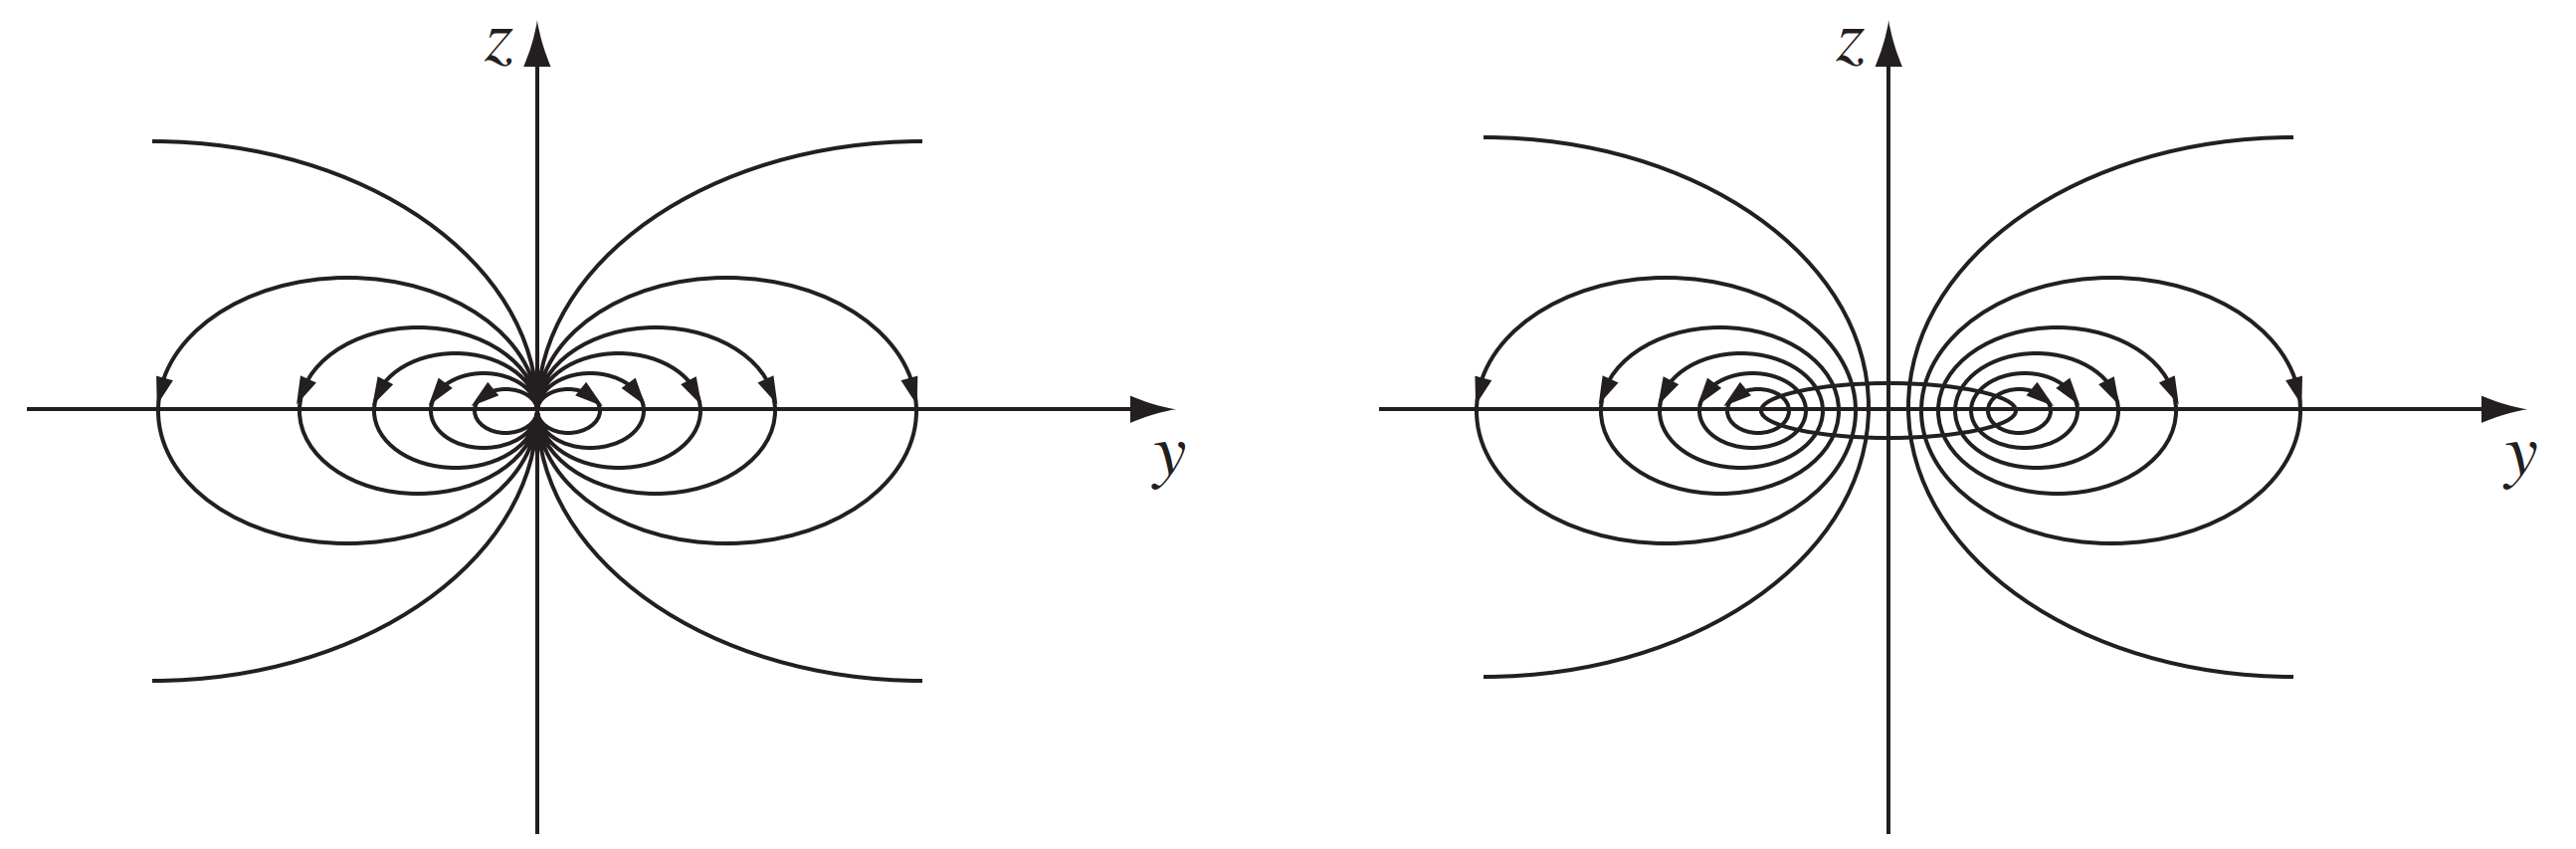
\includegraphics[width=\textwidth]{../Rss/Electromagnetism/Magnetostatics/DipField}
    \caption*{Figure: Field of a "pure" dipole and "physical" dipole}
\end{figure*}

\subsection*{Boundary Condition}
In ELECTROSTATICS, I drew a triangular diagram to summarize the relations among the three fundamental quantities of electrostatics. A similar figure can be constructed for magnetostatics, relating the current density \textbf{J}, the field \textbf{B}, and the potential \textbf{A}.

\begin{figure*}[ht]
    \centering
    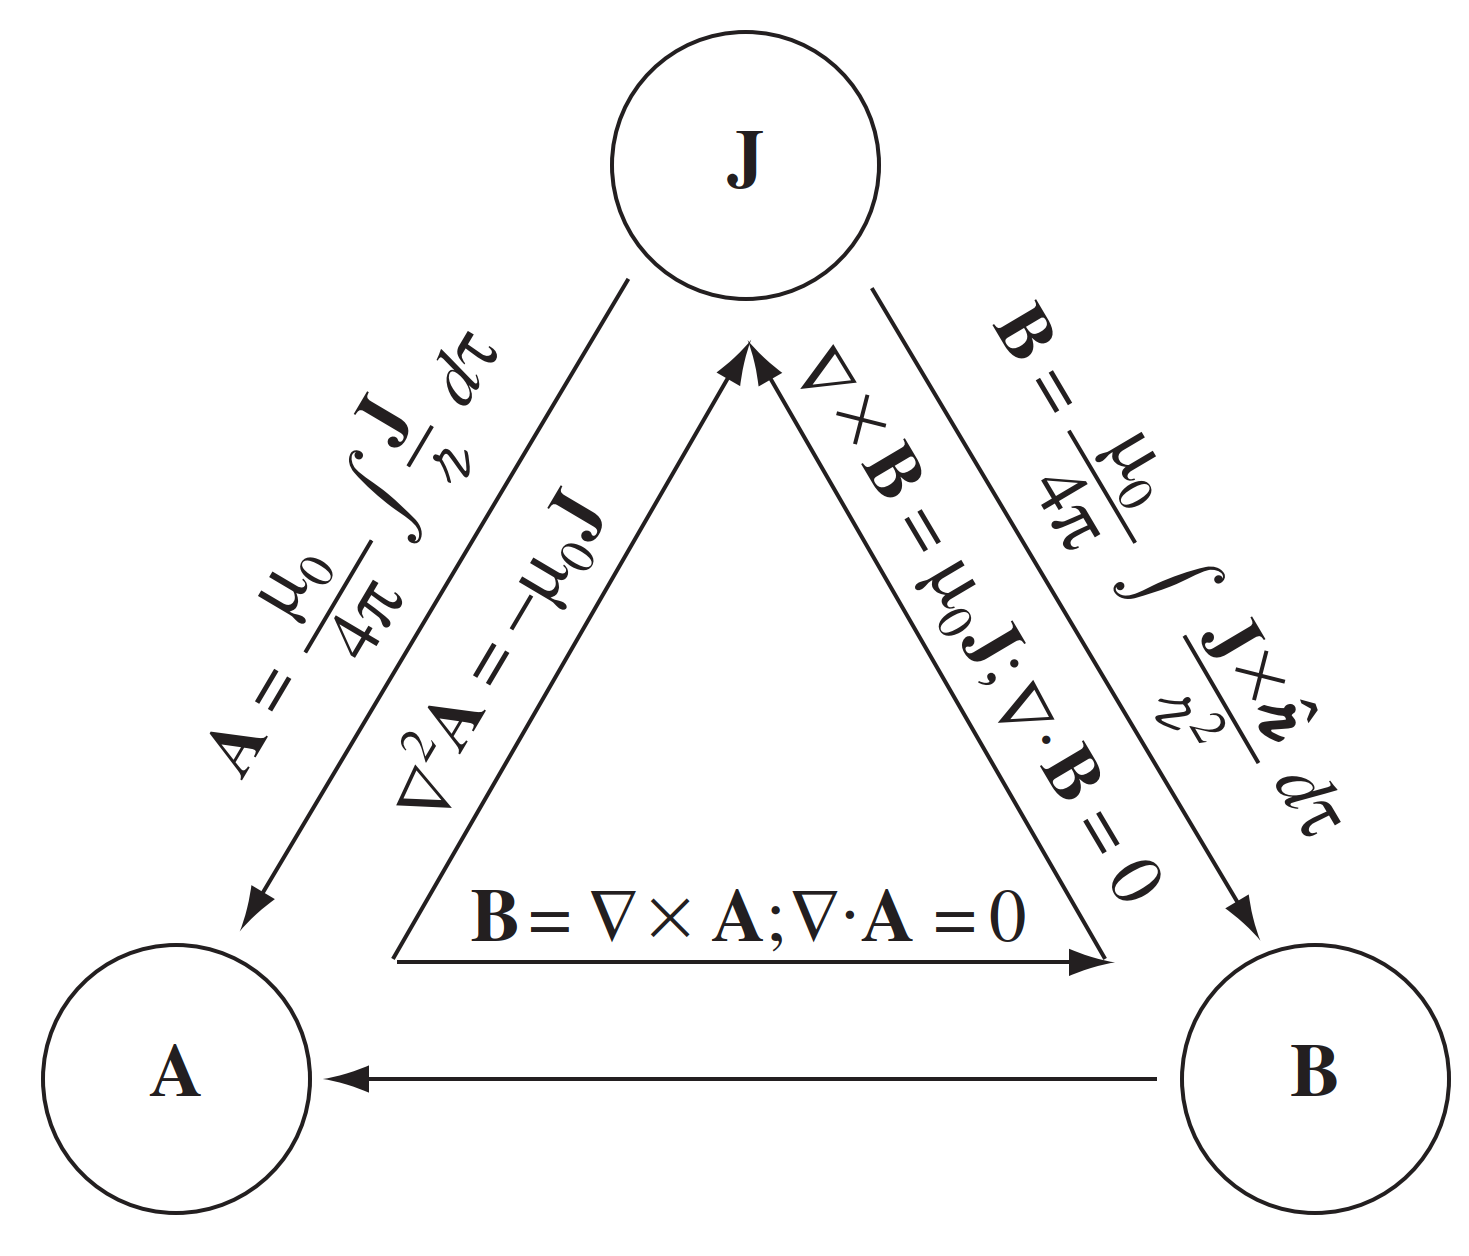
\includegraphics[width=0.5\textwidth]{../Rss/Electromagnetism/Magnetostatics/MagnetostaticsHolyTrinity}
    \caption*{Figure: Magnetostatic Holy Trinity}
\end{figure*}

Just as the electric field suffers a discontinuity at a surface charge, so the magnetic field is discontinuous at a surface current. Only this time it is the tangential component that changes. For perpendicular component
\begin{equation*}
    \mathbf{B}_\text{above}^{\bot}=\mathbf{B}_\text{below}^{\bot}
\end{equation*}
and tangential component
\begin{equation*}
    \mathbf{B}_\text{above}^{||}-\mathbf{B}_\text{below}^{||}=\mu_0K
\end{equation*}

Thus, the component of $\mathbf{B}$ that is parallel to the surface but perpendicular to the current is discontinuous in the amount $\mu_0K$. These results can be summarized in a single formula:
\begin{equation*}
    \mathbf{B}_\text{above}-\mathbf{B}_\text{below}=\mu_0(\mathbf{K}\times\mathbf{\hat{n}})
\end{equation*}

Like the scalar potential in electrostatics, the vector potential is continuous
across any boundary
\begin{equation*}
    \mathbf{A}_\text{above}=\mathbf{A}_\text{below}
\end{equation*}
But the derivative of \textbf{A} inherits the discontinuity of \textbf{B}:
\begin{equation*}
    \frac{\partial \mathbf{A}_\text{above}}{ \partial n}-\frac{\partial \mathbf{A}_\text{below}}{\partial n}= -\mu_0\mathbf{K}
\end{equation*}
\end{document}